\section*{Test 13  Congestion in front of a flight of stairs}

Construct a room that is connected to a flight of stairs by a corridor and occupied as illustrated with a population of adults taken from Figure 5 with an immediate reaction and distribute the walking speeds over a population of 150 persons.

\noindent
The expected result is that congestion will occur at the exit of the room, creating steady flow in the corridor. Additionally, congestion at the foot of the stairs is expected. This will grow over time, as the flow via the stairs is smaller than it is through the corridor.


\begin{figure}[h]
	\centering
	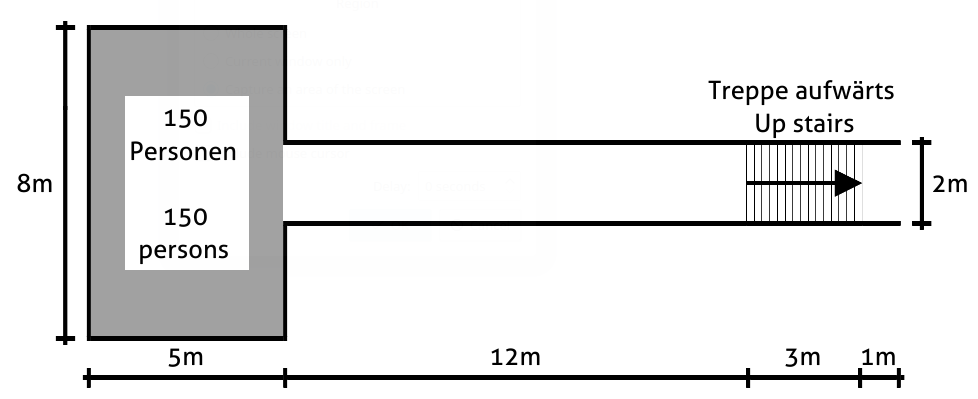
\includegraphics[scale=0.44]{test_description/Escape_route_test_13.png}
	\caption{\footnotesize \textbf{Escape route via stairs
}}
\end{figure}
